\documentclass[a4paper,12pt]{article}

\usepackage[utf8x]{inputenc}
\usepackage[english, russian]{babel}


\usepackage{multirow}
\usepackage{graphicx}
\usepackage{misccorr}
\usepackage{indentfirst}
\usepackage{tabularx}
\usepackage{listings}
\usepackage{xcolor}

\usepackage{fullpage}
\usepackage[labelsep=endash,
		    margin=10pt, 
		    justification = centerlast, 
		    format = hang,
		    singlelinecheck=false
		    ]{caption}

\exhyphenpenalty=10000
\doublehyphendemerits=10000
\finalhyphendemerits=5000

\definecolor{codegreen}{rgb}{0,0.6,0}
\definecolor{codegray}{rgb}{0.5,0.5,0.5}
\definecolor{codepurple}{rgb}{0.58,0,0.82}
\definecolor{backcolour}{rgb}{0.95,0.95,0.92}
 
\lstdefinestyle{mystyle}{
    backgroundcolor=\color{backcolour},
    commentstyle=\color{codegreen},
    keywordstyle=\color{blue},
    numberstyle=\tiny\color{codegray},
    stringstyle=\color{codepurple},
    basicstyle=\footnotesize,
    breakatwhitespace=false,
    breaklines=true,
    captionpos=t,
    keepspaces=true,
    numbers=left,
    numbersep=5pt,
    showspaces=false,
    showstringspaces=false
    showtabs=false,
    tabsize=4,
    frame=tb
}
 
\lstset{style=mystyle}

\usepackage{color}
\usepackage{xcolor}
\usepackage{listings}
 
% Цвета для кода
 
\definecolor{string}{HTML}{B40000} % цвет строк в коде
\definecolor{comment}{HTML}{008000} % цвет комментариев в коде
\definecolor{keyword}{HTML}{1A00FF} % цвет ключевых слов в коде
\definecolor{morecomment}{HTML}{8000FF} % цвет include и других элементов в коде
\definecolor{сaptiontext}{HTML}{FFFFFF} % цвет текста заголовка в коде
\definecolor{сaptionbk}{HTML}{999999} % цвет фона заголовка в коде
\definecolor{bk}{HTML}{FFFFFF} % цвет фона в коде
\definecolor{frame}{HTML}{999999} % цвет рамки в коде
\definecolor{brackets}{HTML}{B40000} % цвет скобок в коде
 

%%% Отображение кода %%%
 
% Настройки отображения кода
 
\lstset{
	% Настройки отображения     
	breaklines=true, % Перенос длинных строк
	% Для отображения русского языка
	extendedchars=true,
	literate={Ö}{{\"O}}1
	{Ä}{{\"A}}1
	{Ü}{{\"U}}1
	{ß}{{\ss}}1
	{ü}{{\"u}}1
	{ä}{{\"a}}1
	{ö}{{\"o}}1
	{~}{{\textasciitilde}}1
	{а}{{\selectfont\char224}}1
	{б}{{\selectfont\char225}}1
	{в}{{\selectfont\char226}}1
	{г}{{\selectfont\char227}}1
	{д}{{\selectfont\char228}}1
	{е}{{\selectfont\char229}}1
	{ё}{{\"e}}1
	{ж}{{\selectfont\char230}}1
	{з}{{\selectfont\char231}}1
	{и}{{\selectfont\char232}}1
	{й}{{\selectfont\char233}}1
	{к}{{\selectfont\char234}}1
	{л}{{\selectfont\char235}}1
	{м}{{\selectfont\char236}}1
	{н}{{\selectfont\char237}}1
	{о}{{\selectfont\char238}}1
	{п}{{\selectfont\char239}}1
	{р}{{\selectfont\char240}}1
	{с}{{\selectfont\char241}}1
	{т}{{\selectfont\char242}}1
	{у}{{\selectfont\char243}}1
	{ф}{{\selectfont\char244}}1
	{х}{{\selectfont\char245}}1
	{ц}{{\selectfont\char246}}1
	{ч}{{\selectfont\char247}}1
	{ш}{{\selectfont\char248}}1
	{щ}{{\selectfont\char249}}1
	{ъ}{{\selectfont\char250}}1
	{ы}{{\selectfont\char251}}1
	{ь}{{\selectfont\char252}}1
	{э}{{\selectfont\char253}}1
	{ю}{{\selectfont\char254}}1
	{я}{{\selectfont\char255}}1
	{А}{{\selectfont\char192}}1
	{Б}{{\selectfont\char193}}1
	{В}{{\selectfont\char194}}1
	{Г}{{\selectfont\char195}}1
	{Д}{{\selectfont\char196}}1
	{Е}{{\selectfont\char197}}1
	{Ё}{{\"E}}1
	{Ж}{{\selectfont\char198}}1
	{З}{{\selectfont\char199}}1
	{И}{{\selectfont\char200}}1
	{Й}{{\selectfont\char201}}1
	{К}{{\selectfont\char202}}1
	{Л}{{\selectfont\char203}}1
	{М}{{\selectfont\char204}}1
	{Н}{{\selectfont\char205}}1
	{О}{{\selectfont\char206}}1
	{П}{{\selectfont\char207}}1
	{Р}{{\selectfont\char208}}1
	{С}{{\selectfont\char209}}1
	{Т}{{\selectfont\char210}}1
	{У}{{\selectfont\char211}}1
	{Ф}{{\selectfont\char212}}1
	{Х}{{\selectfont\char213}}1
	{Ц}{{\selectfont\char214}}1
	{Ч}{{\selectfont\char215}}1
	{Ш}{{\selectfont\char216}}1
	{Щ}{{\selectfont\char217}}1
	{Ъ}{{\selectfont\char218}}1
	{Ы}{{\selectfont\char219}}1
	{Ь}{{\selectfont\char220}}1
	{Э}{{\selectfont\char221}}1
	{Ю}{{\selectfont\char222}}1
	{Я}{{\selectfont\char223}}1
	{і}{{\selectfont\char105}}1
	{ї}{{\selectfont\char168}}1
	{є}{{\selectfont\char185}}1
	{ґ}{{\selectfont\char160}}1
	{І}{{\selectfont\char73}}1
	{Ї}{{\selectfont\char136}}1
	{Є}{{\selectfont\char153}}1
	{Ґ}{{\selectfont\char128}}1
	{\{}{{{\color{brackets}\{}}}1 % Цвет скобок {
	{\}}{{{\color{brackets}\}}}}1 % Цвет скобок }
}


\begin{document}

\begin{titlepage}
\newpage

\

\begin{center}
	\large		
   	Министерство образования и науки Российской Федерации\\[0.5cm]
    	
	ФГБОУ ВПО Рыбинский государственный авиационный технический университет имени П.А. Соловьева\\[1.0cm]

	Факультет радиоэлектроники и информатики\\[0.25cm]
		
	Кафедра математического и программного обеспечения\\ электронных вычислительных средств\\[1.5cm]

	\Large
	\textbf{\textsc{ОТЧЕТ ПО ЛАБОРАТОРНОЙ РАБОТЕ}}\\[0.25cm]
	по  дисциплине\\
	\textbf{Математические методы анализа данных}\\[0.5cm]
	
	по теме\\
	Предварительная обработка значений временных рядов\\ Определение наличия тренда

\end{center}

\vfill	
\begin{tabularx}{0.95\textwidth}{lXr}
Студент группы ИПБ-13 			& &	Иванов Р.А. \\
Преподаватель доцент, к.т.н.	& & Воробьев К. А.\\
\end{tabularx}

\vspace{1.5cm}
\center Рыбинск 2016
\end{titlepage}	

\tableofcontents

\newpage\section{Одномерные гистограммы} 

При выборке размером в 75(рис.~\ref{fig:im2D_1}) можно заметить, что распределение не является равномерным и в целом хотелось бы добиться лучших результатов.
\begin{center}
	\begin{figure}[h]
	    \centering
   		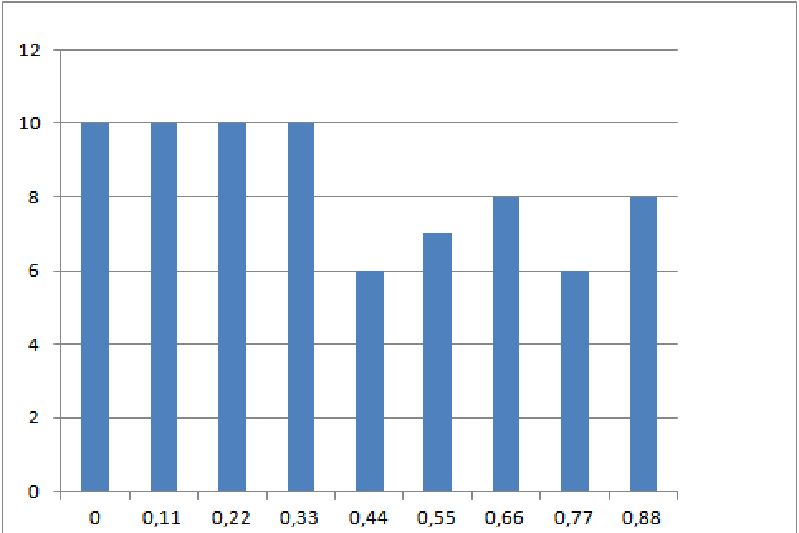
\includegraphics[scale=0.25]{figure_1.png}
   		\caption{одномерная гистограмма для выборки размера 75}
   		\label{fig:im2D_1}
    \end{figure}
\end{center}

При выборке размером в 300(рис.~\ref{fig:im2D_2}) мы можем заметить, что распределение хотя и стало более равномерно, однако, все еще оставляет желать лучшего.
\begin{center}
	\begin{figure}[h]
		\centering
   		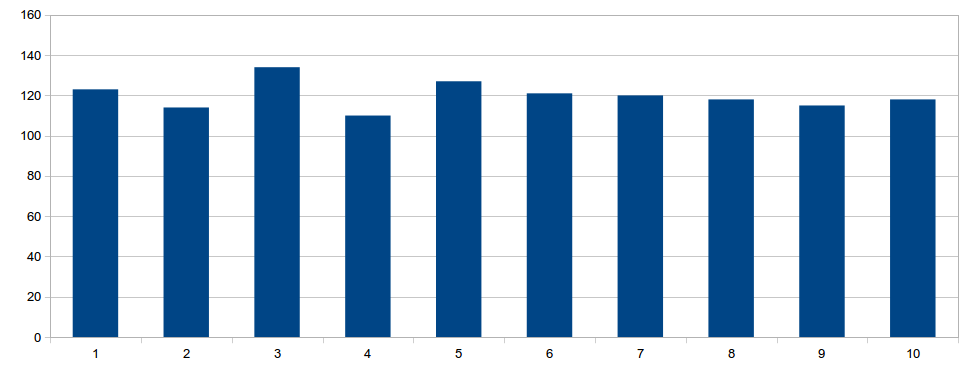
\includegraphics[scale=0.25]{figure_2.png}
   		\caption{одномерная гистограмма для выборки размера 300}
   		\label{fig:im2D_2}
    \end{figure}
\end{center}

При выборке размером в 3000(рис.~\ref{fig:im2D_3}) видно, что распределение начало выравнивать и становить более равномерным, но все еще не идеально.
\begin{center}
	\begin{figure}[h]
		\centering
   		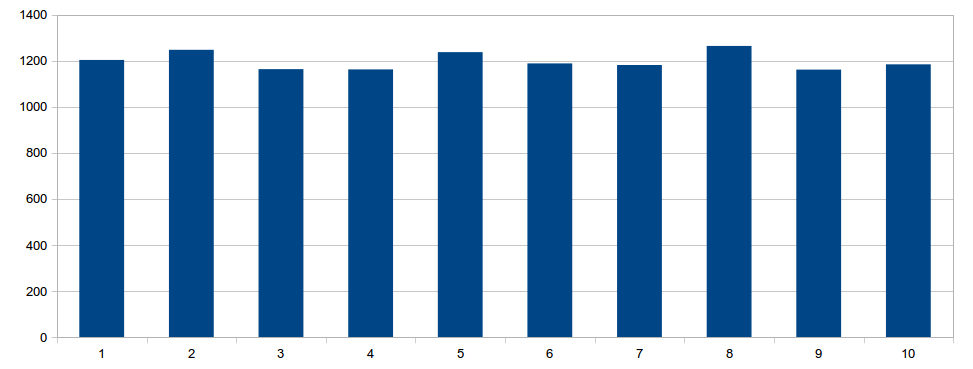
\includegraphics[scale=0.25]{figure_3.png}
   		\caption{одномерная гистограмма для выборки размера 16000}
   		\label{fig:im2D_3}
    \end{figure}
\end{center}

\newpage\section{Двумерные гистограммы} 

При выборке размером 3200(рис.~\ref{fig:im3D_1}), как и в случае с одномерной гистограммой из 3200 реализаций, можно заметить, что существует лишь один отрезкок, в который попало существенно  больше реализаций, чем в какой-либо другой, но равномерность все равно все еще далека от идеальной. Так же мы можем заметить, отсутствие на гистограмме 'волн', т.е. одинаковое количество попаданий в отрезок при переходе по оси Y.
\begin{center}
	\begin{figure}[h]
	    \centering
   		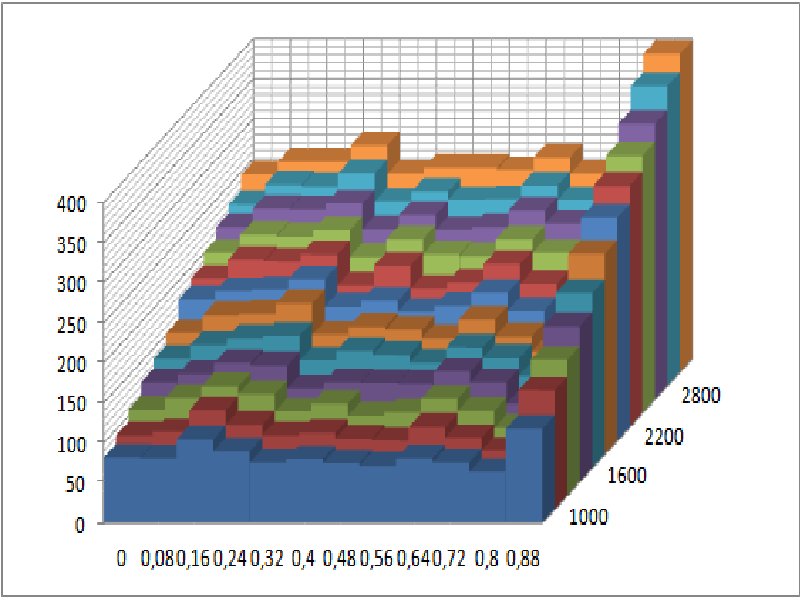
\includegraphics[scale=0.4]{figure_1_1.png}
   		\caption{двумерная гистограмма для выборки размера 3200}
   		\label{fig:im3D_1}
    \end{figure}
\end{center}

Из этого мы можем предположить, что даже значительно увеличение количества реализаций не существенно отразится на гистограмме, хотя и сделает ее более ровной, но все же идеального значения мы не добъёмся.

\newpage\section{Критерий "хи квадрат"}
 
%теперь все подписи будут выравнены по левому ктаю
%т.к. дальше только таблицы
\captionsetup{justification = raggedright}

Критерий $\chi^2$ - это наиболее часто употребляемый критерий для проверки гипотерзы о принадлежности наблюдаемой конечной выборки некоторому теоретическому закону распределения.

{\large $$\chi^2 = \sum\limits_{i=1}^\psi \frac{(n_i - F_i)^2}{F_i}$$}

Для требуемого уровня значимости критическое значение критеря составляет 15.50731. Это значение не было привышено ни для одной исследуемой выборки(таблица~\ref{table:chi}).

\begin{table}[h]
	\caption{вычисленные значения $\chi^2$}
	\begin{tabular}{|c|c|}
	\hline 
	Объём выборки & Значение критерия \\ 
	\hline 
	75 & 2.88 \\ 
	\hline 
	300 & 8.34 \\ 
	\hline 
	30000 & 14.46 \\ 
	\hline 
	\end{tabular}
	
	\label{table:chi}
\end{table}



\newpage\section{Коэффициент автокорреляции}

Автокорреляция — статистическая взаимосвязь между последовательностями величин одного ряда, взятыми со сдвигом. 

{\large $$r = \sum\limits_{i=1}^n \frac{(x_i-0.5)(x_{i+k}-0.5)}{n \ m_2}$$}

В данном случае величина сдвига $k$ равна 4. Значение коэффициента получилось достаточно небльшим (таблица~\ref{table:r}).

\begin{table}[h]
	\caption{вычисленные значения $r$}
	\begin{tabular}{|c|c|}
	\hline 
	Объём выборки & Значение коэффициента \\ 
	\hline 
	75   & 0.17445388175908755   \\ 
	\hline 
	300  & 0.08756757152994353   \\ 
	\hline 
	3000 & 0.0038987736754364675 \\ 
	\hline 
	\end{tabular} 
	\label{table:r}
\end{table}

\newpage\section{Выборочные моменты}

Начальным моментом $k$-го порядка случайной величины $X$ называется математическое ожидание $k$-ой степени этой случайной величины.

{\large $$\alpha_k(X) = M(X^k) = \sum\limits_{i=1}^n x_i^k p_i$$}

Центральным моментом $k$-го порядка случайной величины $X$ называется математическое ожидание $k$-ой степени отклонения случайной величины $X$ от её мат. ожидания.

{\large $$\mu_k(X) = M\left(\left(X-M\left(X\right)\right)^k\right)$$}

Для идеально равномерно распределенной С.В. мат. ожидание должно составлять 0.5, а дисперсия 0.0833333. Представленые ниже рассчетные значения моментов для каждой выборки (таблицы~\ref{table:a_u_1}-\ref{table:a_u_3}) показывают нам, что начальный мемент первого порядка и центральный момент второго порядка с увеличением объёма выборки стремятся к своим идеальнм значениям, что говорит о приближении распределения к идеально равномерному.

\begin{table}[h]
	\caption{вычисленные моменты для выборки объёмом 75}
	\begin{tabular}{|c|c|c|}
	\hline 
	Порядок момента & Начальный момент & Центральный момент \\ 
	\hline 
	1 & 0.4528204517958787 & -9.62193288008469e-18 \\ 
	\hline 
	2 & 0.2904227573920409 & 0.08537639582741716 \\ 
	\hline 
	3 & 0.21410383049348905 & 0.005274110016870604 \\ 
	\hline 
	4 & 0.16927226201211074 & 0.012638636131100205 \\ 
	\hline 
	\end{tabular} 

	\label{table:a_u_1}
\end{table}

\begin{table}[h]
	\caption{вычисленные моменты для выборки объёмом 300}
	\begin{tabular}{|c|c|c|}
	\hline 
	Порядок момента & Начальный момент & Центральный момент \\ 
	\hline 
	1 & 0.4666173320640209 & 4.755455288811087e-17 \\ 
	\hline 
	2 & 0.2979865348135481 & 0.08025480023100331 \\ 
	\hline 
	3 & 0.21703080715779777 & 0.003088563753854017 \\ 
	\hline 
	4 & 0.17001570964008977 & 0.011999790703602275 \\ 
	\hline 
	\end{tabular} 

	\label{table:a_u_2}
\end{table}

\begin{table}[h]
	\caption{вычисленные моменты для выборки объёмом 3000}
	\begin{tabular}{|c|c|c|}
	\hline 
	Порядок момента & Начальный момент & Центральный момент \\ 
	\hline 
	1 & 0.4963843934075088 & -6.938893903907228e-18 \\ 
	\hline 
	2 & 0.3294830339903072 & 0.08308556797176679 \\ 
	\hline 
	3 & 0.24693095913648536 & 8.959646539735148e-4 \\ 
	\hline 
	4 & 0.19772611404316015 & 0.01240299083196629 \\ 
	\hline 
	\end{tabular} 
	
	\label{table:a_u_3}
\end{table}

\newpage\section{Доверительный интервал}
Доверительный интервал $(d)$ уровня $0.95$ определяет интервал, в который с вероятностью $95\%$ попадет мат. ожидание $(\alpha_1)$ элементов выборки.

{\large $$d=t\sqrt{\frac{m_2}{n}}$$}

Где $t$ в данном случае равно 1.96.

Во всех случая мат. ожидания находятся в пределах доверительных интервалов (таблица~\ref{table:d}).

\begin{table}[h]
	\caption{вычисленные значения доверительных интервалов и мат. ожиданий}
	\begin{tabular}{|c|c|c|c|}
	\hline 
	Объём выборки & 0.5 - d & мат. ожидание($a_1$) & 0.5 + d \\ 
	\hline 
	75 & 0.4429802929830179 & 0.08537639582741716 & 0.5570197070169821 \\ 
	\hline 
	300 & 0.47235850131054347 & 0.08025480023100331 & 0.5276414986894565 \\ 
	\hline 
	3000 & 0.49110616897911513 & 0.08308556797176679 & 0.5088938310208849 \\ 
	\hline 
	\end{tabular}
	\label{table:d} 
\end{table}

\newpage\section{Общая оценка качества генератора}
В рассмотренном нами генераторе случайных чисел на основе линейного конгруэнтного метода равномерность распределения увеличивается с увеличением объема выборки. А так же можно увидеть, что значение коэффициента автокорреляции достаточно мало, что говорит нам об отсутствии циклических колебаний случайной велечины с периодичностью 2. Из этого мы можем сделать вывод, что данный метод генерации С.В. удовлетворяет всем предъявляемым требованиям. 


\newpage\section{Приложения}

\begin{lstlisting}[language=Java, title=Генератор случайных чисел]
public class Random {

    public static double a = 8121;
    public static double c = 28411;
    public static int m = 134456;
    public static double seed = 2;

    /**
     * Метод генерирует рандомное число от 0 до 1
     */
    public static double getRand() {
        seed = (a * seed + c) % m;
        return seed / (double) m;
    }

    /**
     * Генерирует рандомное число в диапазоне от a до b
     */
    public static double getRand(int a, int b) {
        return (double) a + ((double) b - (double) a) * getRand();
    }
}


\end{lstlisting}


\begin{lstlisting}[language=Java, title=Рассчет и отображение параметров распределения]
import java.util.ArrayList;
import java.util.List;

import static java.util.stream.Collectors.toList;

/**
 * Класс для вспомогательных вычислений
 *
 * @author Роман
 */
public class CalculationHelper {

    /**
     * Расчитывает математическое ожидание случайной велечины
     *
     * @param list список случайных велечин
     * @return математическое ожидание
     */
    public static double calculateExpectedValue(List<Double> list) {
        double sum = list.stream()
                .mapToDouble(s -> s)
                .sum();
        return sum / list.size();
    }

    /**
     * Расчитать начальный момент случайной велечины
     *
     * @param list список случайныъ велечин
     * @param k степень
     * @return начальный момент
     */
    public static double calculateInitialMoment(List<Double> list, int k) {
        return calculateExpectedValue(list.stream()
                .map(s -> Math.pow(s, k))
                .collect(toList())
        );
    }

    /**
     * Расчитать центральный момент случайной велечины
     *
     * @param list спсок случайных велечин
     * @param k степень
     * @return центральный момент
     */
    public static double calculateCentralMoment(List<Double> list, int k) {
        double expValue = calculateExpectedValue(list);
        return calculateExpectedValue(list.stream()
                .map(s -> Math.pow(s - expValue, k))
                .collect(toList())
        );
    }

    /**
     * Расчитать выборочную дисперсию случайной велечины
     *
     * @param list список случайных велечин
     * @return дисперсия
     */
    public static double calculateDispersion(List<Double> list) {
        return calculateCentralMoment(list, 2);
    }

    /**
     * Посчитать коэффициент автокорелляции
     *
     * @param list список случайных велечин
     * @param k шаг
     * @return коэффициент автокорелляции
     */
    public static double calculateAutocorrelation(List<Double> list, int k) {
        List<Double> forCalculationList
                = list.stream()
                .map(s -> s -= 0.5)
                .collect(toList());
        // количество пар использованых для расчета
        int manyPairs = 0;
        List<Double> resultList = new ArrayList<>();
        for (int i = 0; i < forCalculationList.size(); i++) {
            double mult = forCalculationList.get(i);
            if (i + k < forCalculationList.size()) {
                mult *= forCalculationList.get(i + k);
                manyPairs++;
                resultList.add(mult);
            }
        }

        for (int i = 0; i < resultList.size(); i++) {
            double res = resultList.get(i);
            resultList.set(i, res / manyPairs);
        }

        double sum = resultList.stream()
                .mapToDouble(s -> s)
                .sum();

        return sum / calculateDispersion(list);
    }

    public static double calculateConfidenceInterval(List<Double> list, Double t) {
        return t * Math.sqrt(calculateDispersion(list) / list.size());
    }

\end{lstlisting}


\end{document}
